\documentclass{article}
\usepackage{polski}
\usepackage{textcomp}
\usepackage{amssymb}
\usepackage{float}
\usepackage{cases}
\usepackage[utf8]{inputenc}
\date{2016-10-31}
\usepackage{graphicx}
\author{Szymon Nowak}
\begin{document}
  \section{Teoria}
	  \subsection{Free-space path loss}		  		  
		  Utrata w sile sygnału spowodowana przejściem fali elektromagnetycznej przez ośrodek (najczęściej powietrze).
		  Wzór na obliczanie FSPL:
		  \begin{equation}
			  FSPL = P_{tx} + AG_{tx} + AG_{rx} - P_{rx} - FM - L
		  \end{equation}
		  %http://electronicdesign.com/communications/understanding-wireless-range-calculations
		  %Microwave and Millimetre-Wave Design for Wireless Communications  Autorzy Ian Robertson,Nutapong Somjit,Mitchai str 449
		  %https://en.wikipedia.org/wiki/Free-space_path_loss
		  %http://www.tplink.com/ie/support/calculator/#1
		  %http://stackoverflow.com/questions/11217674/how-to-calculate-distance-from-wifi-router-using-signal-strength
		  Gdzie symbole oznaczają:
		  \begin{itemize}
		  	\item $P_{tx}$ - siła trasmitera, wyrażona w dBm
		  	\item $AG_{tx}$ - zysk energentyczny anteny transmitera, wyrażony w dBi
		  	\item $AG_{rx}$ - zysk energentyczny anteny odbiorcy, wyrażony w dBi
		  	\item $P_{rx}$ - czułość odbiornika, wyrażona w dBm
		  	\item $FM$ - margines zaniku sygnału (fade margin) - określa jak duży jest margines różnicy pomiędzy uzyskaną siłą sygnału, a czułością odbiornika
		  	\item $L$ - straty wynikające np z oddziaływania innych transmiterów, przeszkód itp.
		  \end{itemize}
		  Dodatkowo, FSPL można obliczyć, używając następujący wzór:
		  \begin{equation}
			  FSPL = 20log_{10}\left(\frac{d}{d_{0}}\right) + 20log_{10}(f) + K
		  \end{equation}
		  %Indoor Localization Method Based on Wi-Fi Trilateration Technique Maxim Shchekotov
		  % Wi-Fi Indoor Positioning System Based on RSSI Measurements from Wi-Fi  Access Points  –  A Tri-lateration Approach Onkar Pathak, Pratik Palaskar, Rajesh Palkar, Mayur Tawari
		  Gdzie symbole oznaczają:
		  \begin{itemize}
		  	\item $d$ - dystans dzielący trasmiter od odbiorcy, wyrażony w metrach
		  	\item $d_{0}$ - dystans referencyjny -  w tym wypadku 1 metr
		  	\item $f$ - częstotliwość transmitera - wyrażona w MHz
		  	\item $K$ - stała, którą można określić wzorem:
			  	\begin{equation}
				  	K = 20log_{10}\left(\frac{4\pi d_{0}}{C}\right)
			  	\end{equation}
			  	gdzie $d_{0}$ to dystans referencyjny (taki sam jak we wzorze wyżej), a $C$ to długość fali emitowanej przez transmiter
		  \end{itemize}	  
		  Po przekształceniu wzoru, uzytkujemy:
		  \begin{equation}
			  d = 10^{\left(\frac{FSPL - K - 20log_{10}(f)}{20}\right)}
		  \end{equation}
		  A po połączeniu obu wzorów dostajemy:
		  \begin{equation}
		  d = 10^{\left(\frac{P_{tx} + AG_{tx} + AG_{rx} - P_{rx} - FM - L - K - 20log_{10}(f)}{20}\right)}
		  \end{equation}
		  Dodatkowo, margines zaniku można obliczyć ze wzoru:
		  \begin{equation}
			  FM = P_{rs} - P_{rx}
		  \end{equation}
		  gdzie $P_{rs}$ to siła odebranego sygnału.\\
		  Po podstawieniu powyższego wzoru do wzoru (5), uzyskujemy
		  \begin{equation}
		  d = 10^{\left(\frac{P_{tx} + AG_{tx} + AG_{rx} - P_{rs} - L - K - 20log_{10}(f)}{20}\right)}
		  \end{equation}
		\subsection{Zysk energetyczny anteny}
			Zysk energetyczny anteny jest to stosunek mocy ateny wypromieniowanej w danym kierunku do mocy wypromieniowanej przez antenę wzorcową. Anteną wzorcową może być m.in. antena izotropowa, czyli antena bez fizycznych rozmiarów, która cały sygnał zasilany wysyła we wszystkich kierunkach. W takim wypadku, zysk energetyczny anteny wyrażany jest w $dBi$.\\
			Na zysk energetyczny mają również wpływ kierunkowość oraz materiał, z którego wykonana jest antena.
		\subsection{Received signal strength indication}
			Received signal strength indication (skrótem RSSI) jest to miara określająca moc sygnału odbieranego. Przyjmuje ona wartości niedodatnie (gdzie 0 oznacza sygnał najsilniejszy). Jednostką, w jakiej określa się siłę sygnału jest $dBm$, która jest logarytmiczną jednostką miary mocy odniesiona do mocy $1mW$.\\
			System Android pozwala na odczytanie siły odbieranego sygnału. Można do tego wykorzystać API $WifiManager$ (w przypadku odczytu sygnału WiFi) oraz $BroadcastReceiver$ (w przypadku odczytu sygnału Bluetooth).
		\subsection{Margines zaniku}
	\section{Bluetooth}
		%http://bluetoothinsight.blogspot.com/2008/01/bluetooth-power-classes.html
	\section{Eksperymenty}
		\subsection{Wykorzystane urządzenia}
			\begin{enumerate}
				\item Smartphone Sony Xperia Z1 Compact (D5503) - odbiornik\\				
					Dane techniczne:
					\begin{itemize}
						\item Częstotliwość - 2,4GHz
						\item Przyrost siły sygnału z anteny - 2dBi
					\end{itemize}
				\item Router TP-Link TD-W8970 - nadajnik\\
				Dane techniczne:
				\begin{itemize}
					\item Częstotliwość - 2,4GHz
					\item Dwie zewnętrzne anteny kierunkowe
					\item Przyrost siły sygnału z anteny - 4dBi
					\item Siła transmitera - 16.5dBm					
				\end{itemize}
				\item Router TP-Link TL-WA701ND - nadajnik\\
				Dane techniczne:
				\begin{itemize}
					\item Częstotliwość - 2,4GHz
					\item Jedna zewnętrzna antena kierunkowa
					\item Przyrost siły sygnału z anteny - 2dBi
					\item Siła transmitera - 15dBm					
				\end{itemize}
				\item Smartphone Grand 2 (G7102) - nadajnik\\
				Dane techniczne:
				\begin{itemize}
					\item Częstotliwość - 2,4GHz
					\item Jedna antena wbudowana
					\item Przyrost siły sygnału z anteny - 0dBi
					\item Siła transmitera - 10dBm					
				\end{itemize}
			\end{enumerate}
		\subsection{Warunki}
			Wszystkie pomiary wykonywane były w pomieszczeniu zamknięty, bez przeszkód na drodze sygnału, dlatego jako margines zaniku sygnału została przyjęte wartość 22 dBm. Inne straty (np interferencja sygnałów z routerów) zostały pominięte i ich wykrycie jest jednym z celów eksperymentu.
		\subsection{Cele}
			Celem eksperymentu jest ustalenie, jak zmierzona i obliczona, przy użyciu siły sygnałów, odległość między odbiornikiem i transmiterami odnosi się do odległości rzeczywistej. Dodatkowo, będę się starał ustalić, jak duży wpływ na jakość sygnału mają przeszkody, kierunek, w jakim skierowane są względem siebie urządzenia oraz interferencja sygnałów.
		\subsection{Pomiar odległości}
			Eksperyment polegał na ustawieniu transmitera 1m od odbiornika na jednym poziomie, antenami do siebie. Następnie dodawana była przeszkoda (w tym wypadku książka) i pomiary zostały powtórzone. Eksperyment został wykonany dla wszystkich transmiterów.\\			
			\begin{figure}	
				\centering			
				\caption{Szkic eksperymentu nr 1}
				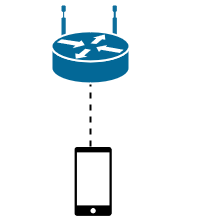
\includegraphics{exper1}
			\end{figure}
			\begin{itemize}
				\item Router TP-Link TD-W8970
				\begin{center}
					\begin{minipage}{\linewidth}
					Wersja bez przeszkody:\\\\
					\begin{tabular}{|c|c|c|}
						\hline 
						Pomiar & Siła sygnału (w dBm) & Obliczona odległość (w metrach) \\ 
						\hline 
						1 & -41 & 1,16 \\ 
						\hline 
						2 & -40 & 1,04 \\ 
						\hline 
						3 & -37 & 0.73 \\ 
						\hline 
						4 & -42 & 1.30 \\ 
						\hline 
						5 & -37 & 0,73 \\ 
						\hline 
					\end{tabular} 
				\end{minipage} 
				\end{center}
				\begin{center}
					\begin{minipage}{\linewidth}
						Wersja z przeszkodą:\\\\
					\begin{tabular}{|c|c|c|}
						\hline 
						Pomiar & Siła sygnału (w dBm) & Obliczona odległość (w metrach) \\ 
						\hline 
						1 & -38 & 0,82 \\ 
						\hline 
						2 & -39 & 0,92 \\ 
						\hline 
						3 & -42 & 1,30 \\ 
						\hline 
						4 & -46 & 2,07 \\ 
						\hline 
						7 & -43 & 1,46 \\ 
						\hline 
					\end{tabular}				
					\end{minipage} 
				\end{center}
			\item Router TP-Link TL-WA701ND
			\begin{center}
				\begin{minipage}{\linewidth}
					Wersja bez przeszkody:\\\\
					\begin{tabular}{|c|c|c|}
						\hline 
						Pomiar & Siła sygnału (w dBm) & Obliczona odległość (w metrach) \\ 
						\hline 
						1 & -44 & 0,98 \\ 
						\hline 
						2 & -44 & 0,98 \\ 
						\hline 
						3 & -45 & 1,10 \\ 
						\hline 
						4 & -47 & 1,38 \\ 
						\hline 
						5 & -45 & 1,10 \\ 
						\hline 
					\end{tabular} 
				\end{minipage} 
			\end{center}
			\begin{center}
				\begin{minipage}{\linewidth}
					Wersja z przeszkodą:\\\\
					\begin{tabular}{|c|c|c|}
						\hline 
						Pomiar & Siła sygnału (w dBm) & Obliczona odległość (w metrach) \\ 
						\hline 
						1 & -49 & 1,74 \\ 
						\hline 
						2 & -47 & 1,38 \\ 
						\hline 
						3 & -46 & 1,23 \\ 
						\hline 
						4 & -47 & 1,38 \\ 
						\hline 
						5 & -47 & 1,38 \\ 
						\hline 
					\end{tabular}//
				\end{minipage} 
			\end{center}
		\item Samsung Grand 2
		\begin{center}
			\begin{minipage}{\linewidth}
				Wersja bez przeszkody:\\\\
				\begin{tabular}{|c|c|c|}
					\hline 
					Pomiar & Siła sygnału (w dBm) & Obliczona odległość (w metrach) \\ 
					\hline 
					1 & -51 & 1,38 \\ 
					\hline 
					2 & -50 & 1,23 \\ 
					\hline 
					3 & -49 & 1,10 \\ 
					\hline 
					4 & -48 & 0,98 \\ 
					\hline 
					5 & -53 & 1,74 \\ 
					\hline 
				\end{tabular} 
			\end{minipage} 
		\end{center}
		\begin{center}
			\begin{minipage}{\linewidth}
				Wersja z przeszkodą:\\\\
				\begin{tabular}{|c|c|c|}
					\hline 
					Pomiar & Siła sygnału (w dBm) & Obliczona odległość (w metrach) \\ 
					\hline 
					1 & -50 & 1,23 \\ 
					\hline 
					2 & -54 & 1,95 \\ 
					\hline 
					3 & -53 & 1,74 \\ 
					\hline 
					4 & -55 & 2,19 \\ 
					\hline 
					5 & -55 & 2,19 \\ 
					\hline 
				\end{tabular}//
			\end{minipage} 
		\end{center}
		\end{itemize}
		
		\subsection{Pomiary zakłóceń}
		Eksperyment polegał na rozmieszczeniu trasmiterów na wierzchołkach trójkąta, w środku którego znajdował się odbiornik. Wszystkie urządzenia znajdowały się na tej samej wysokości. Mierzone były zmiany siły sygnału i obliczonej odległości w zależności od kąta położenia odbiornika w stosunku do trasmitera oraz ilości nakładających się na siebie sygnałów. Na początku, włączony był tylko transmiter o indeksie A. Odbiornik znajdował się w stosunku do transmitera pod kątem około 50 stopni. Następnie włączony został transmiter B. Na końcu do modelu został dodany trasmiter C.\\
		
		\begin{figure}				
			\centering
			\caption{Model systemu do pomiaru zakłóceń}
			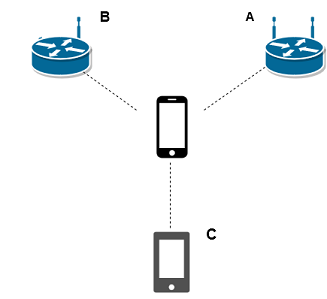
\includegraphics{inz2}
		\end{figure}
		Informacje o urządzeniach:
		\begin{itemize}
			\item Transmiter A - TP-Link TD-W8970, współrzędne (1.80, 0)
			\item Transmiter B - TP-Link TL-WA701ND, współrzędne (0, 0)
			\item Transmiter C - Samsung Grand 2, współrzędne (1.07, 1.8)
			\item Odbiornik - współrzędne (1.2, 0.45)
		\end{itemize}
		\begin{center}
			\begin{minipage}{\linewidth}
				Pomiar bez zakłóceń dla odległości 80cm przy kącie 50\textdegree :\\\\
				\begin{tabular}{|c|c|c|}
					\hline 
					Pomiar & Siła sygnału (w dBm) & Obliczona odległość (w metrach) \\ 
					\hline 
					1 & -41 & 1,16 \\ 
					\hline 
					2 & -43 & 1,46 \\ 
					\hline 
					3 & -41 & 1,16 \\ 
					\hline 
					4 & -42 & 1,30 \\ 
					\hline 
					5 & -43 & 1,46 \\ 
					\hline 
				\end{tabular}
			\end{minipage} 
		\end{center}
		\begin{center}
			\begin{minipage}{\linewidth}
				Pomiar z zakłóceniami z transmitera B dla odległości 80cm przy kącie 50\textdegree :\\\\
				\begin{tabular}{|c|c|c|}
					\hline 
					Pomiar & Siła sygnału (w dBm) & Obliczona odległość (w metrach) \\ 
					\hline 
					1 & -44 & 1,64 \\ 
					\hline 
					2 & -47 & 2,31 \\ 
					\hline 
					3 & -45 & 1,84 \\ 
					\hline 
					4 & -48 & 2,60 \\ 
					\hline 
					5 & -47 & 2,31 \\ 
					\hline 
				\end{tabular}
			\end{minipage} 
		\end{center}
		\begin{center}
			\begin{minipage}{\linewidth}
				Pomiar z zakłóceniami z obu transmiterów dla odległości 80cm przy kącie 50\textdegree :\\\\
				\begin{tabular}{|c|c|c|}
					\hline 
					Pomiar & Siła sygnału (w dBm) & Obliczona odległość (w metrach) \\ 
					\hline 
					1 & -48 & 2,60 \\ 
					\hline 
					2 & -47 & 2,31 \\ 
					\hline 
					3 & -44 & 1,64 \\ 
					\hline 
					4 & -48 & 2,60 \\ 
					\hline 
					5 & -46 & 2,06 \\ 
					\hline 
				\end{tabular}
			\end{minipage} 
		\end{center}
	\subsection{Wyznaczanie lokalizacji użytkownika}
	  Narazie mało do napisania. Z dwóch pomiarów dla modelu z góry, dostałem lokalizacje (-0,4; 1,2; -0,3) oraz (1,5; 1,67; -1,5).
\section{Model wyznaczania lokalizacji}
	Stworzyłem model algorytmu w MatLabie. Nie wyobrażam sobie modelu w trzech wymiarach i z kolorem (według mnie wynikiem będzie prostopadłościan o granatowym dominującym kolorze ścian) , dlatego stworzyłem model 2D, który jest tak naprawdę przekrojem modelu 3D (płaszczyzną XY).
	\begin{figure}	
		\centering			
		\caption{Model systemu z trzema routerami}
		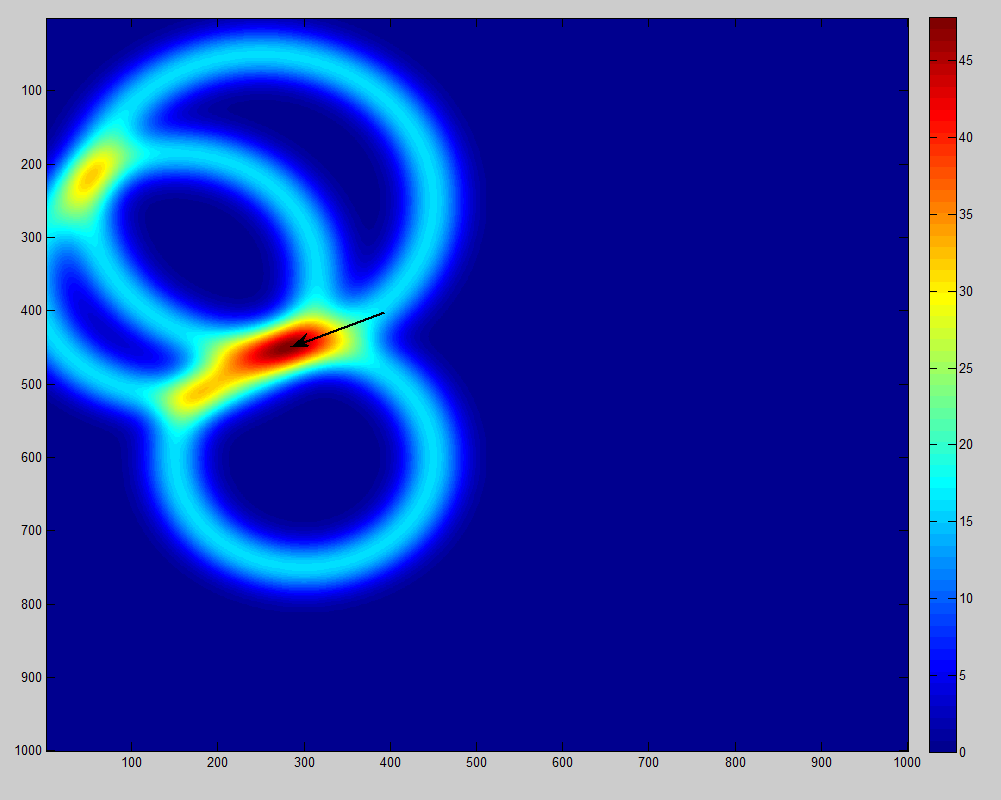
\includegraphics[width=\textwidth]{guasianRouter}
	\end{figure}
	Algorytm zmieniłem według zastrzeżeń Pana Doktora. Prostopadłościan, który zawiera w sobie "sfery" ruterów, dzielony jest na max 20 kawałków. Wyznacza się najlepszą pozycję, dla niej brane są sąsiadujące pozycję i uzyskany sześcian dzieli się na 9 kawałków i ponownie wyznacza najlepszą pozycję. Obliczenia kończą się, jak spełnione jest założenie: $szerKawalka \leqslant okreslonaDokladnosc$.
	
\section{Implementacja}
	\subsection{Serwer}
		Serwer jest aplikacją, która ma analizować zabrane dane, sterować urządzeniami zewnętrznymi oraz stanowić most pomiędzy klientem administracyjnym, a aplikacjami mobilnymi. Na zadania aplikacji serwerowej składają się:
		\begin{itemize}
			\item Zbieranie danych z aplikacji mobilnych oraz wyznaczanie lokalizacji użytkowników
			\item Zezwalanie użytkownikowi administracyjnemu na konfigurację systemu poprzez żądań aplikacji klienckiej
			\item Sterowanie i zarządzanie urządzeniami zewnętrznymi analizując dane odebrane z aplikacji mobilnych
			\item Dostarczanie, w formie skumulowanej lub w czasie rzeczywistym, danych na temat położenia użytkowników do analizy i monitoringu
		\end{itemize}
		\subsubsection{Lokalizacja użytkowników mobilnych}
		\paragraph{Pobranie i analiza danych}
		Serwer pobiera dane od użytkowników w formie requestów HTTP. Każde żądanie wysłane do serwera musi posiadać adres MAC urządzenia Bluetooth wysyłającego oraz listę zarejestrowanych sygnałów. Każda pozycja na liście sygnałów musi posiadać nazwę urządzenia, którego sygnał został odebrany (w przypadku sygnału wysłanego przez router jest to SSID sieci, zaś w przypadku urządzeń Bluetooth jest to adres MAC), typ sygnału (WIFI albo Bluetooth) oraz zarejestrowaną siłę sygnału, określoną w dBm. \\
		Następnie, dla każdego elementu z listy dociągane są stałe dane zarejestrowane w systemi - lokalizacja oraz waga sygnału. Dane na temat routerów oraz stałych urządzeń Bluetooth (np. Beconów) pobierane są bazy danych. Jeżeli jakiś sygnał Bluetooth nie widnieje w bazie danych, sprawdzane są ostatnie żądania od urządzeń mobilnych, dla których udało się określić lokalizacjęa, a czas od ostatniej aktualizacji nie jest większy niż 4 sekundy. Jeżeli sygnał pochodzi od jednego z tych urządzeń, potrzebne informacje pobierane są z dynamicznie budowanej, lokalnej bazy wiedzy. Jeżeli sygnał nie figuruje ani w bazie danych, ani w bazie dynamicznej, zostaje uznany jako sygnał przypadkowy i odrzucony. Waga sygnału przyjmuje wartości w skali od 1 do 4. Domyślnie, sygnałowi pochodzącemu od routera WiFi nadawana jest waga 3, sygnałowi ze stałego urządzenia Bluetooth waga 2, zaś sygnały pochodzące od innych użytkowników mobilnych wagę 1. Wagę stałych urządzeń WiFi i Bluetooth można edytowac przy użyciu panelu konfiguracyjnego w aplikacji klienckiej. W ostatnim kroku, dla każdego zarejestrowanego sygnału obliczana jest odległość urządzenia od użytkownika. Wykorzystywana do tego jest lokalizacja użytkownika, wzór na Free-space path loss oraz dane statyczne (jak siła anten, siła trasmitera itp.).\\
		\paragraph{Algorytmiczne wyznaczenie lokalizacji}
		Celem algorytmu jest wyznaczenie punktu, dla którego suma prawdopodobieństw wynikających z odległości użytkownika od urządzenia, jest największa.\\
		Dane pobrane od użytkownika, uzupełnione o statyczne dane przechowywane w systemie, przekazane są do sekcji napisanej w języku F\#. Na wstępie, do każdego zarejestrownego algorytmu zostaje przypisana probabilistyczna Guassa, określająca prawdopodobieństwo znalezienia się użytkownika w danym punkcie w przestrzeni, gdzie stała $\mu$ przyjmuje wartość równą dystansowi obliczonemu na podstawie siły sygnału urządzenia. Dzięki takiemu podejściu, każdy sygnał można zwizualizować jako sferę, której powierzchnia zbliżona jest do chmury. Największe zagęszczenie prawdopodobieństwa występuję dla średnicy równej odległości obliczonej z siły sygnału, a która rzednie zbliżając się i oddalając od środka sfery.\\
		Pierwszym krokiem algorytmu jest wyznaczenie prostapadłościanu, dla którego wykonywane będą obliczenia. Wielkość bryły dobrana jest tak, aby wewnątrz niej znalazły się wszystkie sfery sygnałów (przy uwzględniu zapasu równego 2$\sigma$). Następnie prostopadłościan oraz sfery są normalizowane w taki sposób, aby początek układu zaczył się w punkcie (0,0,0), zaś wszystkie wartości współrzędnych przyjmowały tylko wartości nieujemne. Celem takiej operacji jest uproszczenie algorytmu oraz wyzbycie się potrzeby skalowania iteratorów oraz odnośników do elementów w tablicach.\\
		Kolejnym krokiem algorytmu jest podział prostopadłościanu na części, dla których liczona będzie suma prawdopodobieństw. Celem tego kroku jest podział pola działania na jednakowe sześciany w takie sposób, aby w żadnym wymiarze ilość sześcianów nie przekroczyła 100. Aby to uzyskać, najdłuższy bok prostopadłościanu zostaje podzielony na 100 częście. Następnie boki w pozostałych 2 wymiarach zostają podzielone na sześciany o krawędziach równej długości. Dzięki takiemu zabiegowi dzieli się prostopadłościan na sześciany. Podział prostopadłościanu na sześciany pozwala na wyeliminowanie błędów obliczeniowych wynikających z nierealistycznego podziału pola oliczeń.\\
		Kolejnym krokiem algorymtu jest wyliczenie sumy prawdopodobieńst ze wszystkich sfer sygnałów dla każdego sześcianu w prostopadłościanie. Każde prawdopodieństo, będące składową sumy, przemnażane jest przez wagę danego sygnału.		
		\begin{equation}
			P(x,y,z) = \sum_{r=1}^{r=R} w_r * \frac{1}{\sigma\sqrt{2\pi}}e^{\left(\frac{-(d-\mu)^2}{2\sigma^2}\right)}
		\end{equation}
		gdzie:
		\begin{itemize}
			\item x, y, z - współrzędne konkretnego sześcianu
			\item R - ilość routerów w modelu
			\item $w_r$ - waga konkretnego routeru
			\item $\sigma$ - odchylenie standardowe, w naszym modelu wynosi: długość najdłuższego boku prostopadłościanu podzielona przez 30
			\item $\mu$ - średnia, w naszym modelu jest to wartość równa, obliczonej na podstawie siły sygnału, odległości użytkownika od źródła sygnału
			\item d - odległość Euklidesowa pomiędzy sześcianem, a routerem
		\end{itemize}
		Następnie wybierany jest sześcian, dla którego suma prawdopodobieństwa jest najwyższa. Jeżeli długość boku sześcianu jest równa lub mniejsza od naszego przybliżenia, współrzędna sześcianu staje się lokalizacją naszego użytkownika. Jeżeli długość boku sześcianu jest większa od naszego przybliżenia, dla wybranego sześcianu dobierane są jego sześciany sąsiednie. Następnie wybrane 27 sześcianów staje się nowym modelem obliczeniowym. Każdy wymiar nowego pola dzialone jest na 9 równych części, dzięki czemu uzyskuje się 729 sześcianów. Algorytm zostaje powtórzony, aż lokalizacja nie zostanie określona z interesującym nas przybliżeniem. Sześcian o największej sumie prawdopodobieństw staje się lokalizacją użytkownika.\\
		Ostatnim krokiem algorytmu jest przeliczenie obliczonej lokalizacji przy użyciu danych uzyskanych podczas normalizacji, aby obliczona lokalizacja odpowiadała lokalizacji dla danych wejściowych.
		\paragraph{Zarządzanie lokalizacją użytkownika}
		Po pozytywnym obliczeniu lokalizacji, zostaje ona zapisana w bazie danych, aby potem mogła być użyta do wyświetlenia skumulowanej mapy przepływu użytkowników albo do sterowania urządzeniami. Następnie, lokalizacja zostaje asynchronicznie wysłana do wszystkich klientów administracyjnych, którzy zarejestrowali swoją chęć pobierania danych w trybie real-time (w czasie rzeczywistym). Następnie, lokalizacja wraz z adresem MAC użytkownika zostaje przekazana do wątków urządzeń zewnętrznych, które wykorzystują te dane do podjęcia decyzji o wywołaniu przypisanego urządzeniowi eventu. W ostatnim kroku, lokalizacja zostaje dodana (lub podmieniona, jeżeli wpis o danym użytkowniku już istnieje) w bazie dynamicznej, aby ta informacja mogła posłużyć przy wyznaczaniu lokalizacji innych użytkowników.
		\subsubsection{Sterowanie i zarządzanie urządzeniami}
		Serwer, poza pobieraniem i analizą danych, zajmuje się również sterowaniem przydzielonymi mu urządzeniami. Sterowanie urządzeniami odbywa się na dwa sposoby:
		\begin{itemize}
			\item Przy użyciu eventów - urządzenia mogą mieć przypisaną klasę obsługującą zdarzenia specjalne. Mechanizm analizuje w czasie rzeczywistym ostatnie zarejestrowane lokalizacje użytkowników, a następnie na ich podstawie, oraz na podstawie wcześniej przypisanych sobie reguł decyduje, czy mają zostać podjętę jakieś działania. Jeżeli tak, komunikuje się z urządzeniem, aby ustawić mu wyznaczone parametry. Wywołana metoda zwraca zmienną typu Boolean, określającą, czy została podjęta decyzja o komunikacji z urządzeniem.
			\item Co określony interwał czasowy - mechanizm, który co jakiś określony czas oblicza parametry, jakie należy przekazać do urządzenia. Robi to na podstawie zarejestrowanych przez ten czas pozycji użytkowników. Do swoich obliczeń wykorzystuje wagi użytkowników, przypisane im w panelu administracyjnym. Mechanizm czasowy ma niższy priorytet niż mechanizm eventów, dlatego jeżeli klasa obsługująca zdarzenia przekazała urządzeniu parametry, system czasowy zostaje zawieszony aż do kolejnego przejścia pętli. Takie rozwiązanie zapobiega nadpisywaniu parametrów wysłanych do urządzenia, zanim wcześniejsze zostaną wykorzystane.
		\end{itemize}
		Informacje na temat urządzeń przechowywane są w bazie danych. Danymi, które są potrzebne do sterowania urządzeniem, niezależnie od jego typu są:
		\begin{itemize}
			\item Jego lokalizacja (określona przez 3 współrzędne)
			\item Ip urządzenia oraz port, na którym nasłuchuje
			\item Nazwę rozpoznawalną przez użytkownika (np żarówka na korytarzu)
			\item Sterownik określający sposób komunikacji, implementujący interfejs przypisany do konkretnego typu urządzenia
			\item Moduł określający, czy dla danego urządzenia przypisane jest jakieś sterowanie eventami (np natychmiastowa zmiana siły oświetlenia, spowodowana zbliżeniem się określonego użytkownika)
			\item Flaga określająca, czy dane urządzenie jest aktywne
		\end{itemize}
		\paragraph{Dobór parametrów sterujących}
		Dla każdego aktywnego urządzenia zapisanego w systemie uruchomiony jest na serwerze osobny wątek sterujący. Taki sposób pracy został przyjęty, aby sterowanie i obsługa eventów odbywała się płynnie i w równy sposób dla wszystkich urządzeń, a błąd czy problemy komunikacyjne jednego z urządzeń nie miały wpływu na inne. Do każdego wątku sterującego przypisany jest obiekt klasy zawierającej wszystkie potrzebne informacje oraz metody, aby kontrolować dany typ urządzenia (dla oświetlenia jest to klasa LightDeviceControllingThread).\\
		Praca wątku polega na wywołaniu metody StartControll(), na której ciało słada się nieskończona pętla while. Niezależnie od typu urządzenia, którym zarządza wątek, każda klasa posiada obiekt kolejki, do której kontroler przyjmujący dane od urządzeń mobilnych wstawia obliczone lokalizacje (pod warunkiem, że dla urządzenia sterowanego przypisano klasę obsługującą zdarzenia).\\
		Kolejnym krokiem, jaki wykonywany jest w metodzie, jest pobranie z kolejki wszystkich oczekujących lokalizacji, a następnie przekazanie ich do klasy sterującej eventami. W systemie zaimplementowana jest przykładowa klasa sterująca światłem - ImportantUserFirstContr. Wybiera z listy użytkowników, którzy są w bliskiej odległości od źródła światła, a następnie wyszukuje wsród nich użytkowników o najwyższej wadze. Jeżeli taki użytkownik zostanie znaleziony, system wysyła do urządzenia rozkaz ustawienia światła o największej mocy. Taki poziom zostanie utrzymany aż ostatni użytkownik uprzywilejowany nie oddali się od źródła światła. System poczeka wtedy dodatkowe 4 sekundy, a następnie wyśle do urządzania informację o ustawieniu mocy światła na poprzednią wartość. System pozwala na rozszerzanie klas sterujących oraz tworzenie swoich i przypisywanie ich urządzeniom (o ile odpowiedni wpis zostanie dodany do bazy danych).\\
		Jeżeli moduł zarządzania eventami zadecyduje o wysłaniu do urządzenia parametrów ustawiających, wykonuje się moduł zarządzania czasowego. Przed wykonaniem obliczeń, algorytm sprawdza, czy od ostatniej czasowej aktualizacji minął odpowiedni okres czasu (domyslnie algorytm ma się wykonywać co godzinę). Data poprzedniej aktualizacji przechowywana jest w polu LastUpdate, które jest aktualizowane obecną datą za każdym razem, jak algorytm pozytywnie wyliczy parametry dla urządzenia. Jeżeli odpowieni czas minął, program pobiera z bazy wszystkie pozycje użytkowników, które zostały zarejestrowane w okresie od ostatniej aktualizacji. Następnie, algorytm wybiera z pobranej listy użytkowników, którzy zostali zarejestrowani w odległości nie większej niż, domyślne, 5 metrów, a nestępnie sumuje ich wagi. Parametr, jaki ma zostać wysłany do urządzenia jest liczony na podstawie wzoru:
		\begin{equation}
		P_{ustalona} = (P_{max} - P_{min}) * \frac{N_{blisk}}{N_{ogół}} + P_{min}
		\end{equation}
		gdzie zmienne w równaniu oznaczają:
		\begin{itemize}
			\item $P_{ustalona}$ - moc światła jaka ma być ustawiona dla urządzenia
			\item $P_{min}$ - minimalna moc światła ustawiona dla urządzenia
			\item $P_{max}$ - maksymalna moc światła ustawiona dla urządzenia
			\item $N_{blisk}$ - suma wag użytkowników, którzy zostali zarejestrowani wystarczająco blisko urządzenia
			\item $N_{ogół}$ - suma wag wszystkich użytkowników w danym okresie czasowym
		\end{itemize}
		Wysyłany parametr jest ustawiany dodatkowo w zmiennej PreviousStaticPowerLevel, aby mógł być potem, w ramach potrzeby, wykorzystany przez moduł sterujący eventami. Na końcu, do zmiennej przechowywującej ostatnią aktualizacje zostaje przypisana obecna data i godzina.\\
		Jeżeli parametry urządzenia zostały zaktualizone w obecnym przebiegu algorytmu, ponowne wykonywanie algorytmu rozpoczyna się od razu. Jeżeli nie, wątek zostaje uśpiony na 0,1 sekundy, aby nie zurzywać niepotrzebnie zasobów serwera.
		\paragraph{Komunikacja z urządzeniami}
		Sposób komunikacji serwera z urządzeniem nie jest zapisany bezpośrednio w kodzie serwera, ale jest przechowywany w bazie danych i przypisywany indywidualnie do konretnego urządzenia. Może zostać zmieniony przy użyciu panelu administracyjnego. Dla każdego typu urządzenia może być zdefiniowana pewna pula modułów komunikacji z urządzeniami. Każdy typ ma określony interfejs, po którym ma dziedziczyć klasa komunikująca się z tego typu urządzeniami. Wewnątrz modułu komunikacyjnego określony jest format wysyłanej wiadomości, kodowanie oraz kolejność parametrów. Ilość metod, które ma udostępniać klasa implementująca interfejs jest zależna od ilości parametrów, jakie mogą być ustawiane w danym typie urządzeń.
		\begin{figure}[H]			
			\centering
			\caption{Model komunikacji z urządzeniami oświetleniowymi}
			\includegraphics[width=1.0\textwidth]{modul_komunikacji}
		\end{figure}
		W systemie został stworzony intefejs ILightDeviceInterface. Powinien być implementowany przez moduły do komunikacyjni z urządzeniami odpowiedzialnymi za oświetlenie. Z racji tego, iż światło posiada tylko jeden sterowalny parametr - moc światła, interfejs narzuca na klasie zaimplementowanie metody NotifyInformationToDevice, która jako parametry przyjmuje ip urządzenia, jego port oraz wartość mocy światła, jaka ma być wysłana do urządzenia. Zadaniem implementacji tej metody jest sformatowanie wiadomości, zawierającej ustawianą moc światła, według standardu urządzenia oraz wysłanie jej protokołem obslugiwanym przez urządzenie. Metoda ma zwrócić zmienną typu Boolean, informującą o tym, czy komunikacja i wysłanie wiadomości się powiodło.\\		
		W ramach przykładu, stworzony został moduł do komunikacji z urządzeniami oświetleniowymi, LoggerLightDeviceInterface. Wysyła on protokołem HTTP na podany adres Ip wiadomość o formacie \textit{"Należy ustawić wartość na: $P_{swiatla}$"}, gdzie $P_{swiatla}$ to moc światła, którą chcemy ustawić.
		\subsubsection{Konfiguracja systemu}
		Aplikacja serwerowa pozwala na konfigurację elementów systemu bez potrzeby jego restartowania. Serwer wykorzystuje do tego kontroler ConfController, przyjmujący żądania HTTP. Podstawowymi elementami, które mogą być konfigurowane w taki sposób są:
		\begin{itemize}
			\item Wielkość pola operacyjnego - wartość określająca, jak duży jest obszar, na którym zainstalowany jest system. Wewnątrz tego pola muszą znajdować się wszystkie obsługiwane routery i urządzenia Bluetooth, ktore nie zmieniają swojej pozycji (np Becony). Jednostką, w jakiej zapisana jest wielkość mapy, są metry. Wartość ta wykorzystywana jest podczas wyświetlania lokalizacji użytkowników w aplikacji administracyjnej - współrzędna lokalizacji zostaje przeskalowana przy użyciu wielkości pola w taki sposób, aby realistycznie odzorowywała położenie na mapie wyświetlanej w aplikacji administracyjnej.
			\item Dane o routerach Wifi i nieporuszających się urządzeniach Bluetooth - administrator systemu ma możliwość zmiany kluczowych danych na temat urządzeń, na podstawie których lokalizowani są potem użytkownicy. Poza danymi technicznymi, dotyczącymi specyfikacji urządzenia (siła trasmitera, siła anten, straty wynikające z kształtu obudowy - np antena wewnętrzna), zdefiniowane są również:
			\begin{itemize}
				\item typ sygnału wysyłanego przez urządzenie - Wifi albo Bluetooth
				\item nazwa, po której urządzenie jest rozpoznawalne przez aplikację mobilną - SSID w przypadku routera WiFi, Mac w przypadku urządzenia Bluetooth
				\item lokalizacja urządzenia - wymagane jest podanie lokalizacji w trzech wymiarach. Współrzędne urządzenia, jak wszystkie współrzędne w systemie, są podawane stosunku punktu określonego jako początek pola działania systemu.
				\item waga urządzenia, która uwzględniana jest podczas lokalizowania użytkownika. Wartość ta podczas dodawania nowego urządzenia, inicjalizowana jest wartościami domyślnymi, które potem można zmienić. Dopuszczalna wartość wagi jest liczbą całkowitą z zakresu $<1:4>$. Domyślne wartości to:
				\begin{itemize}
					\item dla urządzeń Bluetooth, dynamicznie zmieniających swoją pozycję (użytkownicy aplikacji mobilnej) - 1
					\item dla urządzeń Bluetooth, których lokalizacja jest określona - 2
					\item dla urządzeń Wifi - 3
				\end{itemize}
			\end{itemize}
			Dane na temat routerów przechowywane są w bazie danych, skąd są pobierane podczas włączania się aplikacji serwerowej. Informacje te są również przechowywane lokalnie, w pamięci serwera. Ma to na celu zmiejszenie czasu wykonywania operacji, ponieważ pobieranie danych z bazy danych jest dużo wolniejsze niż korzystanie ze zmiennych zapisanych w pamięci. Dlatego, każdorazowa zmiana informacji o routerach powoduje zmianę danych przechowywanych lokalnie przez serwer. System zakłada, że dane o routerach dokonywane są tylko przy użyciu aplikacji serwerowej - zmiany dokonane na bazie przez zewnętrzne aplikacje (np GUI bazy danych) nie zostaną uwzględnione przez serwer aż do jego restartu.
			\item Dane na temat urządzeń sterowanych - podobnie jak w przypadku urządzeń do lokalizacji użytkowników, sterowane urządzenia mogą być dodawane, edytowane oraz usuwane przez administratorów systemu. Informacje różnią się w zależności od kategorii, do której należy dane urządzenie, jednak część z nich jest wspólna:
			\begin{itemize}
				\item nazwa - nazwa urządzenia, która ma pozwolić na jego identyfikację przez użytkowników systemu
				\item ip i port - podstawowe dane wykorzystywane do komunikacji z urządzeniem
				\item lokalizacja - położenie urządzenia określone przez trzy współrzędne
				\item moduł eventów - nazwa modułu, który ma obsługiwać wydarzenia związane z danym urządzeniem. Do urządzenia może nie być przypisany żaden moduł eventów
				\item moduł komunikacyjny - nazwa modułu, który ma pozwolić na komunikację serwera z urządzeniem
				\item czy moduł jest aktywny - informacja ta jest wykorzystywana podczas sterowania urządzeniem 
			\end{itemize}
			Informacje na temat sterowanych urządzeń, poza wpisami w bazie danych, przechowywane są również w pamięci serwera. W przeciwieństwie do routerów (których dane przechowywane są statycznie w klasie SystemDataKnowledge), dane na temat urządzeń znajdują się w przypisanych im obiektach sterujących. Jest to związane z tym, że wątki sterujące są jedynymi elementami aplikacji serwerowej, które często korzystają z tej informacji.\\
			Z racji tego, iż z każdym sterowanym urządzeniem, zarządzanym przez system, związany jest obiekt sterujący, kontroler konfigurujący odpowiedzialny jest również za edycję wątków sterujących. W przypadku dodawania do systemu nowego sterowanego urządzenia, kontroler inicjalizuje nowy obiekt sterujący oraz startuje związany z nim wątek. W przypadku usuwanie urządzenia, kontroler zatrzymuje wątek sterujący i usuwa jego obiekt z listy obiektów sterujących.
			\item Dane na temat użytkowników systemu - kontroler konfiguracyjny pozwala na edycję wagi użytkownika oraz jego nazwy. System rozpoznaje użytkowników po adresie MAC - zmiana nazwy użytkownika ma na celu jedynie pomóc osobie korzystającej z systemu łatwiejsze rozpoznawanie użytkowników. Waga używana jest przy sterowaniu urządzeniami - użytkownik o wadze 4 (przykładowo szef) jest ważniejsza z punktu widzenia modułu określający parametry urządzeń, niż osoba o wadze 1 (zwykły pracownik). Dodatkowo, waga może mieć wpływ na moduły obsługi zdarzeń, przypisany do urządzenia - światło urządzenia może być ustawiane wartością maksymalną w przypadku pojawienia się w okolicy użytkownika o wadze 4.\\
			Dane o użytkownikach przechowywane są w bazie - nie ma potrzeby przechowywania lokalnej kopii.
		\end{itemize}
		Poza konfiguracją systemu, kontroler dostarcza aplikacji administracyjnej danych, potrzebnych do dokonywania zmian w systemie oraz poprawnego działania aplikacji klienckiej. Możliwe jest pobranie danych na temat:
		\begin{itemize}
			\item routerów
			\item typach sygnałów routerów
			\item sterowanych urządzeniach
			\item kategoriach sterowanych urządzeń
			\item dostępnych modułach sterujących eventami
			\item dostępnych modułach komunikacyjnych
			\item wielkości pola działania systemu
			\item użytkownikach
		\end{itemize}
		Dane, w zależności od rodzaju, pobierane są z bazy danych lub lokalnej pamięci serwera.
	\subsubsection{Zarządzanie pozostałymi funkcjami aplikacji administracyjnej}
		Do obsługi pozostałych, poza konfiguracją, żądań aplikacji klienckiej służy kontroler ClientController. Zawiera on metody pozwalające na:
		\begin{itemize}
			\item logowanie i wylogowywanie się użytkownika - użytkownika w momencie włączania aplikacji zmuszony jest do zalogowania się. W momencie logowania, na serwer zostaje wysłane żądanie zawierające jego login. Następnie wysłany login zostaje powiązany z adresem ip, z którego przyszło żądanie. Jest to robione w celu umożliwienia późniejszego wysyłania informacji do klienta bez potrzeby wysłania przez niego żądania - wykorzystywane w momencie, w którym użytkownik zadeklaruje chęć monitorowania użytkowników mobilnych.
			\item pobranie informacji o sterowanych urządzeniach zarejestrowanych w systemie. Ta metoda różni się od metody pobrania urządzeń z kontrolera konfigurującego - lista urządzeń jest pobierana w celu wyświetlenia na mapie. Dodatkowo, pobierane są wszystkie przyrządy, bez względu na ich kategorię. Jedynymi zwracanymi informacjami są lokalizacja urządzenia (w celu wyświetlenia w odpowiednim miejscu) oraz jego kategoria (aby aplikacja kliencka mogła dobrać odpowiednią ikonkę).
			\item zgłoszenie żądania zapisania użytkownika do subskrypcji lokalizacji użytkowników - system zostaje poinformowany, że dany administrator chce monitorować wszystkich pojawiających się użytkowników aplikacji mobilnej. W momencie określenia lokalizacji użytkownika, do wszystkich użytkowników, na adres ip pobrany podczas logowania, zostaje wysłana notyfikacja zawierająca współrzędne użytkownika oraz jego adres MAC.
			\item pobranie lokalizacji użytkowników z danego okresu czasowego - administrator zgłasza chęć pobrania wszystkich lokalizacji, które zostały zarejestrowane w podanym przez niego okresie czasu. W odpowiedzi, do osoby żądającej, wysłana zostaje lista zawierająca współrzędne lokalizacji użytkowników oraz ich adresy MAC.
		\end{itemize}	
	\subsection{Aplikacja administracyjna}
		Głównym celem aplikacji klienckiej jest konfiguracja systemu i wyświetlanie oraz monitorowanie lokalizacji użytkowników. Dostęp do niej powinien być ograniczony, ze względów bezpieczeństwa, wyłącznie do uprzywilejowanych użytkowników.
		\subsubsection{Opis okien aplikacji}
		\paragraph{Okno logowania}
		Pierwszym oknem, które pojawia się po włączeniu aplikacji, jest okno logowania. Osoba upoważniona wprowadza swój login oraz hasło. Naciśnięcie przycisku "Zaloguj" powoduje wysłanie zapytania do aplikacji serwerowej, która tworzy lokalny wpis o logowaniu się użytkownika oraz przechowuje adres IP, z którego przyszło żądanie. Zapisany adres wykorzystywany jest m.in. do wysyłania powiadomień o pojawieniu się lokalizacji mobilnej w sytuacji, gdy użytkownik zapiszę się na subskrypcję notyfikacji.\\
		\begin{figure}[H]			
			\centering
			\caption{Okno logowania użytkownika administracyjnego}
			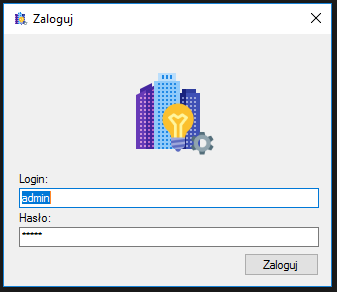
\includegraphics{okno_logowania}
		\end{figure}
		Po pozytywnym przejściu procesu logowania, użytkownik zostaje przeniesiony do głównego okna aplikacji. Składa się ono z panelu z mapą, panelu wyboru trybu wyświetlania lokalizacji użytkowników oraz przycisku przejścia do konfiguracji.\\
		\begin{figure}[H]			
			\centering
			\caption{Główne okno aplikacji administracyjnej}
			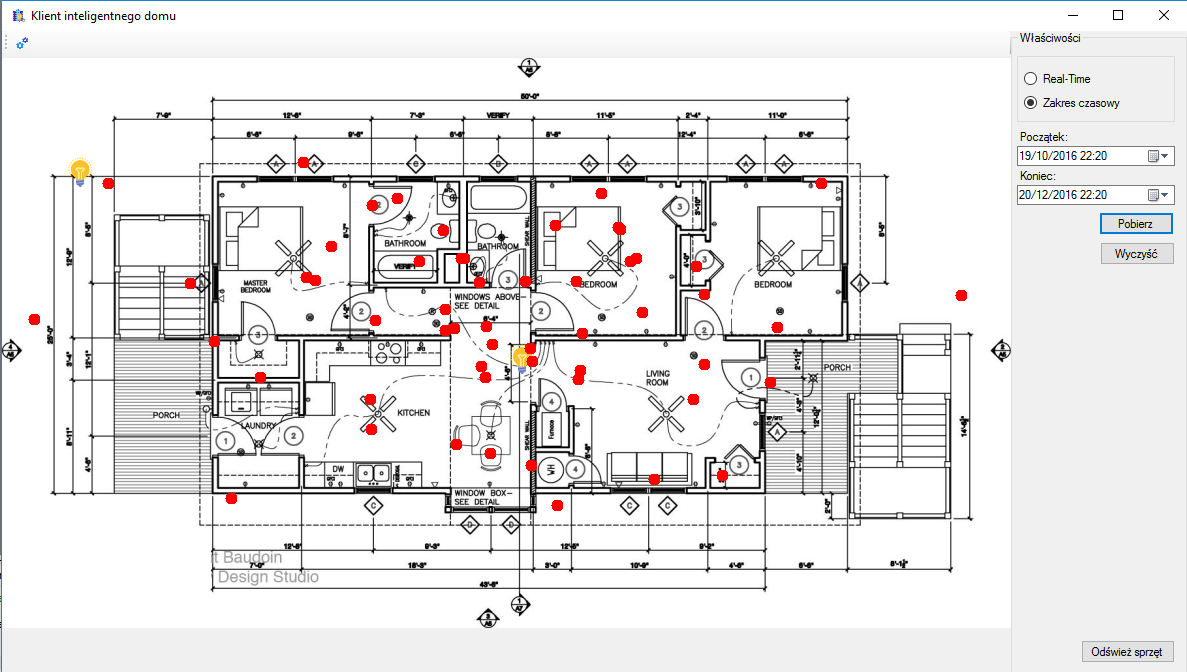
\includegraphics[width=1.0\textwidth]{okno_glowne}
		\end{figure}
		\paragraph{Główne okno}
		W głównym panelu wyświetlana jest mapa systemu, do której ścieżka określona jest w pliku konfiguracyjnym "conf.xml". Jedynym wymaganiem co do mapy jest to, aby była ona plikiem graficznym. Mapa jest skalowalna - każda zmiana wielkości okna powoduje dopasowanie się obrazka do nowego panelu. To samo dotyczy wyświetlanych wewnątrz elementów. Na mapę nanoszone są urządzenia sterowane oraz lokalizacje użytkowników mobilnych. Urządzenia oznaczane są symbolem ich kategorii, zaś użytkownicy reprezentowani są przez czerwone kropki.\\
		Lokalizacje urządzeń pobierane są podczas załadowania aplikacji (jednak po poprawnym przejściu procesu logowania) oraz automatycznie wyświetlane. Z racji tego, iż zmiany w konfiguracji urządzeń przez innych użytkowników administracyjnych nie odświeżają ikon na mapie, w prawym dolnym rogu aplikacji znajduje się przycisk, którego naciśnięcie spowoduje ponowne pobranie z serwera lokalizacji sprzętów sterowanych oraz przerysowanie symboli na mapie.\\
		Lokalizacje użytkowników mobilnych mogą być wyświetlane w dwóch trybach:
		\begin{itemize}
			\item w czasie rzeczywistym - aplikacja administracyjna zgłasza na serwerze chęć zapisania się na subskrypcję lokalizacji. Dzięki temu, za każdym razem, jak tylko serwer ustali lokalizację użytkownika, zostaną o tym powiadomione wszystkie zalogowane aplikacje administracyjne. Punkty oznaczające użytkownika wyświetlane są na okres 4 sekund.
			\item w formie skumulowanej - administrator wysyła na serwer zakres czasowy, dla którego chce wyświetlić pozycje użytkowników. Aplikacja serwerowa pobiera lokalizacje z bazy, a następnie wysyła je spowrotem do klienta, na którym zostają wyświetlone. Punkty oznaczające użytkownika wyświetlane są bez określonego okresu ważności.
		\end{itemize}
		Przejście pomiędzy trybami powoduje usunięcie zachowanych w pamięci lokalizacji.\\
		Punkty reprezentujące użytkowników oraz ikony sprzętów sterowanych są skalowane, aby realistycznie odwzorowywać swoją rzeczywistą pozycję. Wykorzystuje się do tego podane podczas konfiguracji wielkości rzeczywistego obiektu.\\
		Jeżeli stosunek wysokości mapy do jej szerokości jest większy niż stosunek wysokości panelu wyświetlającego mapę do jego szerokości, pozycję ikony w panelu oblicza się na podstawie wzoru:
		\begin{equation}
			\left\{
				\begin{array}{l}
					x = \frac{rzecz\_lok\_urz\_x}{rzecz\_szer\_mapy} * szer\_pan\_mapy \\
					y = \frac{(rzecz\_lok\_urz\_y}{rzecz\_wys\_mapy} * wys\_przel\_mapy + wys\_marg 
				\end{array}
			\right.
		\end{equation}
		gdzie:
		\begin{itemize}
			\item $x$ i $y$ oznaczają współrzędne w panelu mapy
			\item $rzecz\_lok\_urze\_x$ i $rzecz\_lok\_urze\_y$ to fizyczne współrzędne użytkownika mobilnego lub urządzenia sterowanego
			\item $rzecz\_szer\_mapy$ i $rzecz\_wys\_mapy$ to rzeczywiste wymiary prostokąta, wewnątrz którego znajduje się system
			\item $szer\_pan\_mapy$ jest to szerokość panelu wyświetlającego mapę (w tym wypadku szerokość mapy i szerokość panelu jest taka sama)
			\item $wys\_przel\_mapy$ to wysokość mapy. W tym wypadku wysykość mapy nie jest równa wysokości panelu - aby zachować realistyczne proporcję, powyżej i poniżej obrazku mapy dodany jest margines. Wysokość mapy obliczana jest ze wzoru:
			\begin{equation}
				wys\_przel\_mapy = \frac{szer\_pan\_mapy * wys\_obraz\_mapy}{szer\_obraz\_mapy}
			\end{equation}
			w którym $wys\_obraz\_mapy$ i $szer\_obraz\_mapy$ to wymiary obrazka mapy, określone w pikselach.
			\item $wys\_marg$ to wysokość marginesu, jaki musi zostać dodany, aby zachować proporcję mapy. Obliczny jest ze wzoru:
			\begin{equation}
				wys\_marg = \frac{wys\_pan\_mapy - wes\_przel\_mapy}{2}
			\end{equation}
		\end{itemize}
		W przypadku, jeżeli stosunek wysokości mapy do jej szerokości jest niższy niż stosunek wysokości panelu wyświetlającego mapę do jego szerokości, obliczenia wykonuje się analogicznie, ale z tą różnicą, że w tym wypadku to wysokość mapy będzie równa wysokości panelu i dlatego to faktyczna szerokość mapy w oknie oraz szerokość bocznych marginesów muszą zostać wyliczone.
		\paragraph{Okno konfiguracji}
		Wciśnięcie przycisku "Konfiguracja" (reprezentowane w oknie jako ikona dwóch trybów), otwiera osobne okno, pozwalające na konfigurację kluczowych elementów systemu.\\
		Pierwszy panel w oknie konfiguracji pozwala na edycję wielkości fizycznej systemu oraz danych na temat routerów (umożliwia ich również dodawanie oraz usuwanie).
		W dolnej części okna wyświetlone są wszystkie zarejestrowane routery. Wciśnięcie wybranego z nich powoduje przejście do trybu edycji - pola edycji routerów zostaną wypełnione danymi wybranego urządzenia.
		\begin{figure}[H]			
			\centering
			\caption{Panel edycji danych routerów}
			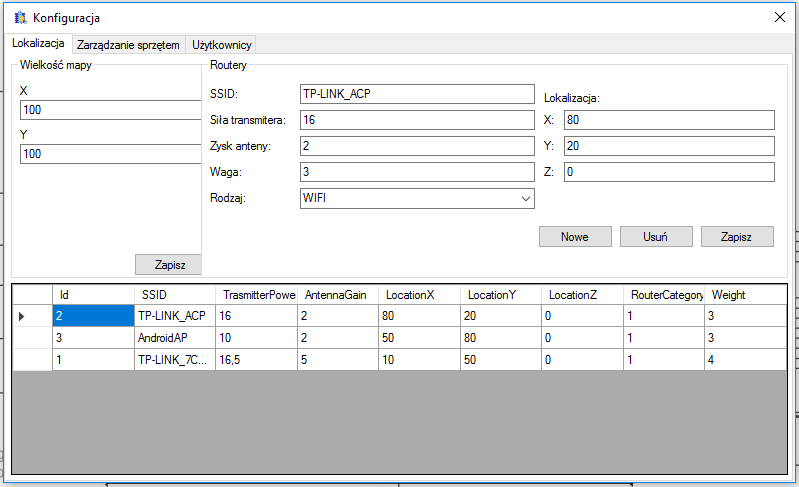
\includegraphics[width=1.0\textwidth]{panel_konf_router}
		\end{figure}
		Poza polami wymaganymi do lokalizacji użytkownika, którymi są:
		\begin{itemize}
			\item lokalizacja routera - współrzędne X, Y, Z oraz SSID
			\item zysk anteny
			\item siła transmitera
		\end{itemize}
		aplikacja pozwala dodatkowo na zadeklarowanie typu sygnału wysyłanego przez urządzenie. Ma to wpływ na sposób obliczania odległości do użytkowników, ale także na wartość początkową wagi przydzielonej temu transmiterowi. Wagę można zmienić ręcznie, ale trzeba pamiętać, że musi się znaleźć w zakresie <1:4>.\\
		Drugi panel pozwala na definiowanie i edycję urządzeń sterowanych.
		\begin{figure}[H]			
			\centering
			\caption{Panel edycji urządzeń sterowanych}
			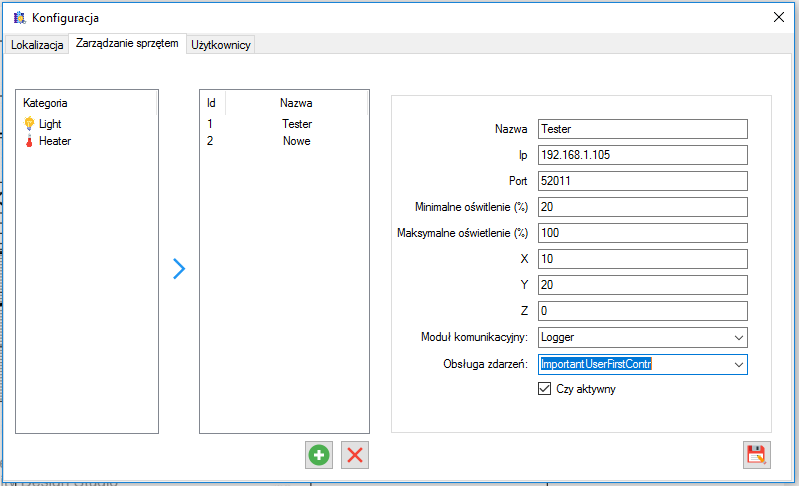
\includegraphics[width=1.0\textwidth]{panel_konf_ster}
		\end{figure}
		Wszystkie urządzenia zarejestrowane w systemi podzielone są na kategorie. Dostępne kategorie przechowywane są w bazie danych i stamtąd są pobierane, kiedy aplikacja klientowa wyśle żądanie na serwer. Wybranie kategorii z lewego panelu powoduje pobranie z serwera wszystkich urządzeń, które należą do wybranej kategorii. Do każdej kategorii przydzielona jest inna akcja w kontrolerze ConfController na serwerze - przykładowo, dla urządzeń oświetleniowych, jest to akcja GetLightDevices.\\
		Aby przejść do widoku wyświetlania i edycji danych urządzenia, należy wybrać interesującą nas pozycję ze środkowego panelu. Powoduje to pojawienie się w prawym panelu formularza z danymi danego urządzenia. Formularze są tworzone dynamicznie, a rodzaj i ilość ich pól zależne są od kategorii urządzenia. Dla urządzenia z kategorii "Światło", dostępne są następujące pola:
		\begin{itemize}
			\item lokalizacji - współrzędne XYZ urządzenia. pozwalające umiejscowić je w rzeczywistym środowisku
			\item adres ip i port - pozwalają na komunikację z urządzeniem
			\item nazwa - pozwala użytkownikom odróżniać urządzenia między sobą
			\item minimalne i maksymalne oświetlenie - zakres, określony w procentach, z którego może korzystać system podczas sterowania urządzeniem. W przypadku sterowania w interwałach czasowych, minimalne oświetlenie przydzielane jest w sytuacji, gdy, w podanym okresie czasu, obok urządzenia nie przeszedł żaden użytkownik. Analogicznie, maksymalne oświetlenie przydzielane jest, gdy wszystkie obliczone lokalizacje użytkowników znajdowały się w niedalekiej odległości od sterowanego urządzenia
			\item moduł komunikacyjny - określa sterownik, sposób komunikacji serwera z urządzeniem. Moduły komunikacyjne definiowane są w bazie danych, a związane z nimi klasy obsługujące muszą zostać dodane do kodu serwera
			\item obsługa zdarzeń - nazwa modułu, który na bieżąco steruje urządzeniem, w zależności od lokalizacji użytkowników zlokalizowanych w bliskiej odległości. Z modułem związana jest klasa, która obsługuje przypisany do urządzenia moduł
		\end{itemize}
		Panel udostępnia przyciski, które pozwalają na zapis wprowadzonych zmian, jak również dodanie lub usunięcie urządzenia.\\
		Ostatni panel to panel użytkowników. Są to osoby, które korzystały z aplikacji mobilnej, a ich pozycja została chociaż raz obliczona.
		\begin{figure}[H]			
			\centering
			\caption{Panel edycji urządzeń sterowanych}
			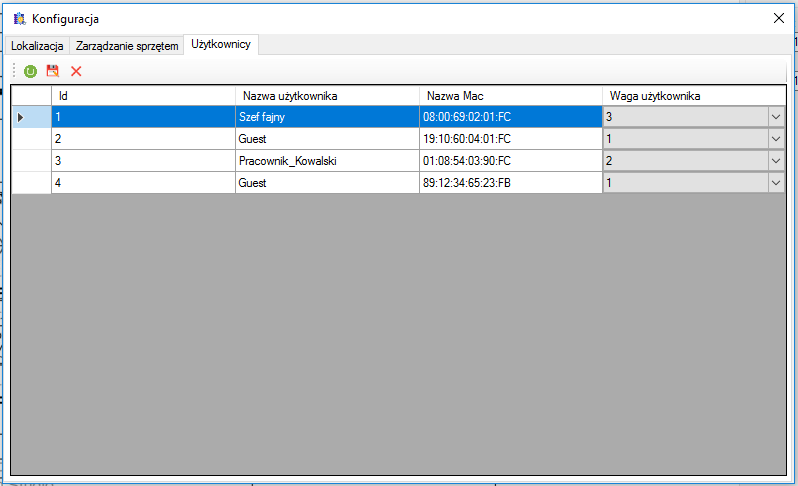
\includegraphics[width=1.0\textwidth]{panel_konf_users}
		\end{figure}
		Okno składa się z tabeli, w której znajdują się zapisani użytkownicy oraz przycisków:
		\begin{itemize}
			\item odświeżania danych
			\item zapisania wszystkich użytkowników
			\item usunięcia wybranego w tabeli użytkownika
		\end{itemize}
		Widok pozwala na podglądnięcie użytkowników oraz na zmianę ich nazwy oraz wagi. Nazwa pozwala na rózróżnianie użytkowników w sposób łatwiejszy niż po adresie MAC. Waga odgrywa kluczową rolę podczas obliczania parametrów do sterowania urządzeniami - czym wyższa waga użytkownika, tym większe ma on znaczenie dla urządzenia, w którego pobliżu znajduje się obliczona lokalizacja. Dodatkowo, pojawienie się użytkownika o określonej wadze może mieć wpływ na zajście, zdefiniowanego dla urządzenia, zdarzenia. Wagi przyjmują wartość od 0 (użytkownik o najniższym priorytecie, nie brany pod uwagę podczas określania parametrów) do 4 (użytkownik o najwyższym priorytecie).
		\paragraph{Wyświetlanie lokalizacji użytkowników} W trybie wyświetlania lokalizacji w czasie rzeczywistym, aplikacja musi wyświetlać uzyskane dane bez odświeżania czy ingerencji użytkownika. 
\end{document}











